
%% bare_conf.tex
%% V1.4b
%% 2015/08/26
%% by Michael Shell
%% See:
%% http://www.michaelshell.org/
%% for current contact information.
%%
%% This is a skeleton file demonstrating the use of IEEEtran.cls
%% (requires IEEEtran.cls version 1.8b or later) with an IEEE
%% conference paper.
%%
%% Support sites:
%% http://www.michaelshell.org/tex/ieeetran/
%% http://www.ctan.org/pkg/ieeetran
%% and
%% http://www.ieee.org/

%%*************************************************************************
%% Legal Notice:
%% This code is offered as-is without any warranty either expressed or
%% implied; without even the implied warranty of MERCHANTABILITY or
%% FITNESS FOR A PARTICULAR PURPOSE! 
%% User assumes all risk.
%% In no event shall the IEEE or any contributor to this code be liable for
%% any damages or losses, including, but not limited to, incidental,
%% consequential, or any other damages, resulting from the use or misuse
%% of any information contained here.
%%
%% All comments are the opinions of their respective authors and are not
%% necessarily endorsed by the IEEE.
%%
%% This work is distributed under the LaTeX Project Public License (LPPL)
%% ( http://www.latex-project.org/ ) version 1.3, and may be freely used,
%% distributed and modified. A copy of the LPPL, version 1.3, is included
%% in the base LaTeX documentation of all distributions of LaTeX released
%% 2003/12/01 or later.
%% Retain all contribution notices and credits.
%% ** Modified files should be clearly indicated as such, including  **
%% ** renaming them and changing author support contact information. **
%%*************************************************************************


% *** Authors should verify (and, if needed, correct) their LaTeX system  ***
% *** with the testflow diagnostic prior to trusting their LaTeX platform ***
% *** with production work. The IEEE's font choices and paper sizes can   ***
% *** trigger bugs that do not appear when using other class files.       ***                          ***
% The testflow support page is at:
% http://www.michaelshell.org/tex/testflow/



\documentclass[conference]{IEEEtran}



\usepackage{graphicx}
\usepackage{subfigure}
\usepackage{graphicx}
\usepackage{caption}

% Some Computer Society conferences also require the compsoc mode option,
% but others use the standard conference format.
%
% If IEEEtran.cls has not been installed into the LaTeX system files,
% manually specify the path to it like:
% \documentclass[conference]{../sty/IEEEtran}





% Some very useful LaTeX packages include:
% (uncomment the ones you want to load)


% *** MISC UTILITY PACKAGES ***
%
%\usepackage{ifpdf}
% Heiko Oberdiek's ifpdf.sty is very useful if you need conditional
% compilation based on whether the output is pdf or dvi.
% usage:
% \ifpdf
%   % pdf code
% \else
%   % dvi code
% \fi
% The latest version of ifpdf.sty can be obtained from:
% http://www.ctan.org/pkg/ifpdf
% Also, note that IEEEtran.cls V1.7 and later provides a builtin
% \ifCLASSINFOpdf conditional that works the same way.
% When switching from latex to pdflatex and vice-versa, the compiler may
% have to be run twice to clear warning/error messages.






% *** CITATION PACKAGES ***
%
%\usepackage{cite}
% cite.sty was written by Donald Arseneau
% V1.6 and later of IEEEtran pre-defines the format of the cite.sty package
% \cite{} output to follow that of the IEEE. Loading the cite package will
% result in citation numbers being automatically sorted and properly
% "compressed/ranged". e.g., [1], [9], [2], [7], [5], [6] without using
% cite.sty will become [1], [2], [5]--[7], [9] using cite.sty. cite.sty's
% \cite will automatically add leading space, if needed. Use cite.sty's
% noadjust option (cite.sty V3.8 and later) if you want to turn this off
% such as if a citation ever needs to be enclosed in parenthesis.
% cite.sty is already installed on most LaTeX systems. Be sure and use
% version 5.0 (2009-03-20) and later if using hyperref.sty.
% The latest version can be obtained at:
% http://www.ctan.org/pkg/cite
% The documentation is contained in the cite.sty file itself.






% *** GRAPHICS RELATED PACKAGES ***
%
\ifCLASSINFOpdf
  % \usepackage[pdftex]{graphicx}
  % declare the path(s) where your graphic files are
  % \graphicspath{{../pdf/}{../jpeg/}}
  % and their extensions so you won't have to specify these with
  % every instance of \includegraphics
  % \DeclareGraphicsExtensions{.pdf,.jpeg,.png}
\else
  % or other class option (dvipsone, dvipdf, if not using dvips). graphicx
  % will default to the driver specified in the system graphics.cfg if no
  % driver is specified.
  % \usepackage[dvips]{graphicx}
  % declare the path(s) where your graphic files are
  % \graphicspath{{../eps/}}
  % and their extensions so you won't have to specify these with
  % every instance of \includegraphics
  % \DeclareGraphicsExtensions{.eps}
\fi
% graphicx was written by David Carlisle and Sebastian Rahtz. It is
% required if you want graphics, photos, etc. graphicx.sty is already
% installed on most LaTeX systems. The latest version and documentation
% can be obtained at: 
% http://www.ctan.org/pkg/graphicx
% Another good source of documentation is "Using Imported Graphics in
% LaTeX2e" by Keith Reckdahl which can be found at:
% http://www.ctan.org/pkg/epslatex
%
% latex, and pdflatex in dvi mode, support graphics in encapsulated
% postscript (.eps) format. pdflatex in pdf mode supports graphics
% in .pdf, .jpeg, .png and .mps (metapost) formats. Users should ensure
% that all non-photo figures use a vector format (.eps, .pdf, .mps) and
% not a bitmapped formats (.jpeg, .png). The IEEE frowns on bitmapped formats
% which can result in "jaggedy"/blurry rendering of lines and letters as
% well as large increases in file sizes.
%
% You can find documentation about the pdfTeX application at:
% http://www.tug.org/applications/pdftex





% *** MATH PACKAGES ***
%
%\usepackage{amsmath}
% A popular package from the American Mathematical Society that provides
% many useful and powerful commands for dealing with mathematics.
%
% Note that the amsmath package sets \interdisplaylinepenalty to 10000
% thus preventing page breaks from occurring within multiline equations. Use:
%\interdisplaylinepenalty=2500
% after loading amsmath to restore such page breaks as IEEEtran.cls normally
% does. amsmath.sty is already installed on most LaTeX systems. The latest
% version and documentation can be obtained at:
% http://www.ctan.org/pkg/amsmath





% *** SPECIALIZED LIST PACKAGES ***
%
%\usepackage{algorithmic}
% algorithmic.sty was written by Peter Williams and Rogerio Brito.
% This package provides an algorithmic environment fo describing algorithms.
% You can use the algorithmic environment in-text or within a figure
% environment to provide for a floating algorithm. Do NOT use the algorithm
% floating environment provided by algorithm.sty (by the same authors) or
% algorithm2e.sty (by Christophe Fiorio) as the IEEE does not use dedicated
% algorithm float types and packages that provide these will not provide
% correct IEEE style captions. The latest version and documentation of
% algorithmic.sty can be obtained at:
% http://www.ctan.org/pkg/algorithms
% Also of interest may be the (relatively newer and more customizable)
% algorithmicx.sty package by Szasz Janos:
% http://www.ctan.org/pkg/algorithmicx




% *** ALIGNMENT PACKAGES ***
%
%\usepackage{array}
% Frank Mittelbach's and David Carlisle's array.sty patches and improves
% the standard LaTeX2e array and tabular environments to provide better
% appearance and additional user controls. As the default LaTeX2e table
% generation code is lacking to the point of almost being broken with
% respect to the quality of the end results, all users are strongly
% advised to use an enhanced (at the very least that provided by array.sty)
% set of table tools. array.sty is already installed on most systems. The
% latest version and documentation can be obtained at:
% http://www.ctan.org/pkg/array


% IEEEtran contains the IEEEeqnarray family of commands that can be used to
% generate multiline equations as well as matrices, tables, etc., of high
% quality.




% *** SUBFIGURE PACKAGES ***
%\ifCLASSOPTIONcompsoc
%  \usepackage[caption=false,font=normalsize,labelfont=sf,textfont=sf]{subfig}
%\else
%  \usepackage[caption=false,font=footnotesize]{subfig}
%\fi
% subfig.sty, written by Steven Douglas Cochran, is the modern replacement
% for subfigure.sty, the latter of which is no longer maintained and is
% incompatible with some LaTeX packages including fixltx2e. However,
% subfig.sty requires and automatically loads Axel Sommerfeldt's caption.sty
% which will override IEEEtran.cls' handling of captions and this will result
% in non-IEEE style figure/table captions. To prevent this problem, be sure
% and invoke subfig.sty's "caption=false" package option (available since
% subfig.sty version 1.3, 2005/06/28) as this is will preserve IEEEtran.cls
% handling of captions.
% Note that the Computer Society format requires a larger sans serif font
% than the serif footnote size font used in traditional IEEE formatting
% and thus the need to invoke different subfig.sty package options depending
% on whether compsoc mode has been enabled.
%
% The latest version and documentation of subfig.sty can be obtained at:
% http://www.ctan.org/pkg/subfig




% *** FLOAT PACKAGES ***
%
%\usepackage{fixltx2e}
% fixltx2e, the successor to the earlier fix2col.sty, was written by
% Frank Mittelbach and David Carlisle. This package corrects a few problems
% in the LaTeX2e kernel, the most notable of which is that in current
% LaTeX2e releases, the ordering of single and double column floats is not
% guaranteed to be preserved. Thus, an unpatched LaTeX2e can allow a
% single column figure to be placed prior to an earlier double column
% figure.
% Be aware that LaTeX2e kernels dated 2015 and later have fixltx2e.sty's
% corrections already built into the system in which case a warning will
% be issued if an attempt is made to load fixltx2e.sty as it is no longer
% needed.
% The latest version and documentation can be found at:
% http://www.ctan.org/pkg/fixltx2e


%\usepackage{stfloats}
% stfloats.sty was written by Sigitas Tolusis. This package gives LaTeX2e
% the ability to do double column floats at the bottom of the page as well
% as the top. (e.g., "\begin{figure*}[!b]" is not normally possible in
% LaTeX2e). It also provides a command:
%\fnbelowfloat
% to enable the placement of footnotes below bottom floats (the standard
% LaTeX2e kernel puts them above bottom floats). This is an invasive package
% which rewrites many portions of the LaTeX2e float routines. It may not work
% with other packages that modify the LaTeX2e float routines. The latest
% version and documentation can be obtained at:
% http://www.ctan.org/pkg/stfloats
% Do not use the stfloats baselinefloat ability as the IEEE does not allow
% \baselineskip to stretch. Authors submitting work to the IEEE should note
% that the IEEE rarely uses double column equations and that authors should try
% to avoid such use. Do not be tempted to use the cuted.sty or midfloat.sty
% packages (also by Sigitas Tolusis) as the IEEE does not format its papers in
% such ways.
% Do not attempt to use stfloats with fixltx2e as they are incompatible.
% Instead, use Morten Hogholm'a dblfloatfix which combines the features
% of both fixltx2e and stfloats:
%
% \usepackage{dblfloatfix}
% The latest version can be found at:
% http://www.ctan.org/pkg/dblfloatfix




% *** PDF, URL AND HYPERLINK PACKAGES ***
%
%\usepackage{url}
% url.sty was written by Donald Arseneau. It provides better support for
% handling and breaking URLs. url.sty is already installed on most LaTeX
% systems. The latest version and documentation can be obtained at:
% http://www.ctan.org/pkg/url
% Basically, \url{my_url_here}.




% *** Do not adjust lengths that control margins, column widths, etc. ***
% *** Do not use packages that alter fonts (such as pslatex).         ***
% There should be no need to do such things with IEEEtran.cls V1.6 and later.
% (Unless specifically asked to do so by the journal or conference you plan
% to submit to, of course. )


% correct bad hyphenation here
\hyphenation{op-tical net-works semi-conduc-tor}


\begin{document}
%
% paper title
% Titles are generally capitalized except for words such as a, an, and, as,
% at, but, by, for, in, nor, of, on, or, the, to and up, which are usually
% not capitalized unless they are the first or last word of the title.
% Linebreaks \\ can be used within to get better formatting as desired.
% Do not put math or special symbols in the title.
\title{Distributed Online Training Simulation for Railway Dispatcher }


% author names and affiliations
% use a multiple column layout for up to three different
% affiliations
\author{\IEEEauthorblockN{Nuri Ozalp, Ahmet Basgoze, Ozdemir Kavak, Burcu Kalkan}
\IEEEauthorblockA{TUBITAK BILGEM\\Informatics and Information Security\\ Research Center\\
Kocaeli, Turkey 41470\\
Email: {(nuri.ozalp, ahmet.basgoze, ozdemir.kavak, burcu.kalkan)}@tubitak.gov.tr}


}

% conference papers do not typically use \thanks and this command
% is locked out in conference mode. If really needed, such as for
% the acknowledgment of grants, issue a \IEEEoverridecommandlockouts
% after \documentclass

% for over three affiliations, or if they all won't fit within the width
% of the page, use this alternative format:
% 
%\author{\IEEEauthorblockN{Michael Shell\IEEEauthorrefmark{1},
%Homer Simpson\IEEEauthorrefmark{2},
%James Kirk\IEEEauthorrefmark{3}, 
%Montgomery Scott\IEEEauthorrefmark{3} and
%Eldon Tyrell\IEEEauthorrefmark{4}}
%\IEEEauthorblockA{\IEEEauthorrefmark{1}School of Electrical and Computer Engineering\\
%Georgia Institute of Technology,
%Atlanta, Georgia 30332--0250\\ Email: see http://www.michaelshell.org/contact.html}
%\IEEEauthorblockA{\IEEEauthorrefmark{2}Twentieth Century Fox, Springfield, USA\\
%Email: homer@thesimpsons.com}
%\IEEEauthorblockA{\IEEEauthorrefmark{3}Starfleet Academy, San Francisco, California 96678-2391\\
%Telephone: (800) 555--1212, Fax: (888) 555--1212}
%\IEEEauthorblockA{\IEEEauthorrefmark{4}Tyrell Inc., 123 Replicant Street, Los Angeles, California 90210--4321}}




% use for special paper notices
%\IEEEspecialpapernotice{(Invited Paper)}




% make the title area
\maketitle

% As a general rule, do not put math, special symbols or citations
% in the abstract
\begin{abstract}
Computer Simulations can be considered as a powerful tools for learning such as analysing, designing, and interacting. Especially in the vital criticality level it has become more important tools such as train traffic simulation.
The most important purpose of the train control system to prevent train collisions with other trains, keeping them in safe range.

The purpose of this study is to provide train traffic control in a distributed simulation system. The system consists of an instructor five students and a scenario-editor. The system use real train route model located in Turkey.  During the simulation, dispatchers console can controls train traffic which have different  size and speed in system. Success in educational outcomes can be measured. Instructor console make decisions about the organization of teaching and learning 
experiences, classroom management, and responses to 
individual students. The user is able to monitor and track the progress of five targeted students throughout the course of the simulation. 
\end{abstract}

\section{INTRODUCTION}
Kara ve Demiryolu taşımacılığında önemli bir yeri bulunan tren, bir ya da birkaç lokomotif tarafından çekilen, itilen ve vagonlardan oluşan bir ulaşım aracıdır. Ulaşım ve taşımacılık anlanlarında trenlerin çok önemli bir yere sahip olduğu bilinen bir gerçektir. 
Artan demiryolu trafiği sonucunda Dünya genelinde değişik trafik kontrol sistemleri geliştirilmiştir. Tren trafiği yönetim metotlarının dünyada birçok farklı merkezi tren trafik kontrol sistemleri vardır.

Demiryolu trafiği yönetimi için kullanılan sistemler merkezi kontrol sistemleri olup, kontrolörler (dispeçer) tarafında idare edilmektedir.  Dispeçerlerin amaçları trenleri güvenle ve zamanında varması gereken hedeflere ulaştırmaktır.

Tren trafiği kontrol sistemleri çok kritik sistemlerdir.Anlık konum bilgisi eski model trenlerde bilinmemektedir. Sinyalizasyon sistemleri sayesinde trenlerin yaklaşık konumları 3km civarında tahmin edilebilmektedir. Bu nedenle tren trafiği kritik olmaktadır. Son yıllarda dispeçer eğitimi sefer sayılarının artması ve tren yollarının artması ile daha da önem kazanmıştır. Dispeçerlerin gerçek tren trfiği üzerinde çalışarak tecrübe kazanmaları hemuzun zaman almakta hem de birtakım riskleri beraberinde getirmektedir. Bu nedenle eğitim simülasyon sistemlerine ihtiyaç duyulmaktadır ve birçok eğitim simulasyonu geliştirilmiştir. Özellikle kontrol merkezlerinde birden çok dipeçerin birlikte çalışmasından dolayı dağıtık yapılı ve birden çok kullanıcılı simulasyonlar önem kazanmıştır. Bu sayede tek bir simulasyonda hazırlanan yoğun trafikli senaryo ile birden çok dispeçerin birlikte tren trafiği yönetmesi ve birçok problemle başa çıkması önem arz etmektedir. 

Bu çalışmada dispeçerlerin geliştirilen simülasyon sistemi altyapısı kullanılarak eğitilmesi ve gerçek tren trafiği yönetimine hazır hale getirilmesi ve daha kısa sürede alanında uzmanlaşabilmesi hedeflenmiştir. Simülasyon ortamında yoğun trafikli, farklı tip ve hızlardaki trenlerin bulunduğu demiryolu sahası oluşturularak bu saha üzerinde meydana gelebilecek problemler oluşturulmakta ve yapılan tüm bu işlemler senaryo olarak kaydedilmektedir. Kaydedilen senoryolar eğitmen tarafından açılarak aynı anda 5 öğrenciye kadar eğitim verilmesine ve sonrasında öğrencilerin performanslarının  değerlendirilerek karne verilmesine imkan sağlamaktadır.

Geliştirilen simülasyon sistemi 5 modülden oluşmaktadır. 
Bunlar; 
. eğitmen konsolu, 
. öğrenci konsolu, 
. seneryo editörü, 
. performans değerlendirme modülü,
. tren graf modülüdür. 

Seneryo editörü ile istenilen arazi hazırlanmakta ve istenilen bütün koşullar bu arazide oluşturulmakta ve istediği kadar değişik konumlarda tren eklenebilmektedir. Eğitmen ister tek simülasyon isterse farklı 5 simülasyon aynı anda başlatabilmekte ve simülasyonlara müdahele edebilmektedir. İstediği zaman snapshot ile eğitimde bazı önemli gördüğü yerleri tekrar tekrar öğrencilere tecrübe ettirebilmektedir. Öğrenciler yetkileri ölçüsünde sorumlu olduğu alanda tren trafiğini yönetebilmekte ve meydana gelen arızaların çözümü için çalışmalar yapabilmektedir. Anlık tren hareketlerini aynı zamanda trengraf ile takip edebilmektedir. Eğitim sonunda değerlendirme yapılabilmekte ve yetiştirilen dispeçerin başarısı ölçülebilmektedir.

2. bölümde related wwork, 3. bölümde sistemin nasıl haberleşme alt yapısı hakkında bilgi verilmiştir. 4. Bölümde sisteme ait 5 modülden bahsedilmiştir. 5. modülde yapılan deney hakkında bilgiler yer almaktadır. 6.  bölümde ise sonuç kısmına yer verilmiştir.


\section{RELATED WORK}

Tren trafiğini yöneten ve birden çok dispeçerin eğitim aldığı dağıtık yapılı simülasyonlar henüz yaygın olarak kullanılmaktadır. Bizim yaptığımız çalışmaya benzer çalışmalara bu bölümde yer verilmiştir.

In Middelkoop and his friend study is a simulator which which stands for Flexible Rail Infra Simulation of Operations (FRISO). It includes automatized  a simulation model by using a connection to database, editor including generator functions and the possibility to perform single and multiple (stochastic) simulation experiments. FRISO models include following elements  track layout, signalling system, route setting, and interlocking. Our system presents multiple screen of regions and to let five students to work at same or different simulation at the same time \cite{FRISO}.

 


In Baohua  and his friend's study is about  multi-train simulator. It is able to do  train performances assessment at the given railway lines, signal layouts optimization, energy-efficient operating strategies , in major terminals exploration of traffic bottlenecks, the evaluation of the reliability of scheduled timetables and train delay propagation. In multi-train simulation does these automatically, in our system dispatcher conduct them \cite{ICVES}.




\section{SYSTEM DESIGN}
\subsection{Simülasyon Yaşam Döngüsü}

RAYTES sistemi beş bağımsız simülasyon ortamını eşzamanlı ve birbirinden bağımsız olarak yürütebilmektedir. Aşağıdaki gösterilen Şekil \ref{fig:simyasamdongusu}' deki yaşam döngüsü bir simülasyon ortamını temsil etmektedir. Sistem ilk çalıştırıldğında IDLE durumda bulunmaktadır. Bir senaryo sisteme yüklenerek simülasyon oturumu oluşturulduğunda LOADED durumuna geçilir. Bu durumda simülasyon başlangiç saatinde beklemekte olup, çalışmaya hazır haldedir. Simülasyon çalıştırıldığında RUNNING durumuna geçer, simülasyon saati ilerlemekte, simüle edilen nesneler zamana duyarlı biçimde işlenir, ve insan arayüzlerinde sistem ile kullanıcılar arası etkileşim gerçeklenmektedir. PAUSE durumunda simülasyon saati ve simülasyon işlemler geçici olarak durdurulur. PAUSE durumunda yine simülasyon RUNNING durumuna başlayabilir. Simülasyon sonlandırıldığında TERMINATED durumuna düşer ve simülasyon artık yeniden başlatılamaz.




\begin{figure}[h!]
  \centering
  % Requires \usepackage{graphicx}
  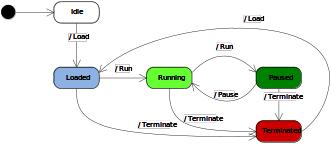
\includegraphics[width=8cm]{simyasamdongusu.jpg}
  \caption{Representation of Simulation Life cycle}\label{fig:simyasamdongusu}
\end{figure}

\subsection{Comminication}
\subsubsection{ Simulation Message}
Simulation Message mesaj türü simülasyon sistemin üst seviye kumanda ve kontrol mesajlaşma türüdür. Bu mesajlar Eğitmen Konsolu’nda üretilmektedir ve sistemin diğer bileşenlerine gönderilmektedir. Simülasyon’un yaratılması, duraklatılması, snapshot alınması, gibi temel simülasyon komutlar içermektedir. Ayrıca simülasyondaki sanal saha nesnelerinin durumlarına müdahale etmek amacıyla bir takım özel müdahale komutlar tanımlıdır. Mesaj komutları Tablo 1 de verilmektedir.
\subsubsection{Request Message}
RequestMessage mesaj türü Kontrol Merkezi Client (KMC) modülünün Kontrol Merkezi Sunucu (KMS) modülüne gönderilen komutları taşımaktadır. KMC ve KMS arasındaki protokol “client-server” mimarisi olup RequestMessage komutları istemci tarafın sunucu tarafından hizmet isteği olarak değerlendirilmektedir. RequestMessage komutları de listelenmektedir.

\subsubsection{State Message}

StateMessage mesajlar simülasyon çalışması esnasında sanal saha daki tanımlı elemanların durum bilgilerinin iletilmesi için kullanılmaktadır. Kontrol Merkezi Sunucu (KMS) modülü StateMessage kullanlarak Kontrol Merkezi Client (KMC) modülüne saha bilgilerini göndermektedir. Kontrol Merkezi Sunucu ayriyetten saha görüntüleme ihtiyacı duyan Geniş Ekran Konsolu (GEK) ve Eğitmen Saha Müdahale (ESM) modüllerine de StateMessage vasıtasıyla bilgi göndermektedir.

\subsubsection{System Message}
SystemMessage mesajlar Öğrenci Kontrol Yönetimi (ÖKY) ile Kontrol Merkezi Sunucu (KMS) modüller arası kullanılan mesajlaşmadır. Bu mesaj türü öğrenci kullanıcıların eğitim sistemine giriş (login) sağlamakta kullanılmaktadır.

\subsection{Modbus}
Modbus otomasyon senayi çevrelerinde kabul görmüş bir ham veri iletişim protokolu. Bu protokol “client-server” mantığında çalışıp sistemler arası bit dizilerin sorgulanması ve iletilmesinde kullanılmaktadır. RAYTES projesinde Modbus paketler UDP/IP üzerinden yazılım modülünden modüle iletilmektedir. Kontrol Merkezi Sunucu (KMS) modülü, Anklaşman Simülatör (AS) modülü, Saha Simülatör (SS) modülü ve Tren Simülatör (TS) modüller arası komut ve bilge transferi Modbus paketler ile gerçekleşmektedir.


\subsection{SSY Simülasyon Sunucu Yönetim Modülü}
SSY yani Simülasyon Sunucu Yönetim modülü simülasyon sistemi içerisindeki tüm aktif modüllerin bağlı olduğu  haberleşme altyapısının ve koordinasyonun sağlandığı modüldür.Şekil \ref{fig:syySequenceDiagram}'de squance diagram ve  Şekil \ref{fig:syygrafic}'de arayüzü gösterilmiştir.
Simülasyon akışı içerisinde doğrudan bir görevle sorumlu tüm aktif modüller bu modüle ya doğrudan ya da altında çalıştıkları ana modül üzerinden dolaylı olarak bağlı olmak zorundadır. Simülasyonun çalışması ve hazırlanması esnasında gerçekleşen tüm mesajlaşmalar bu modül üzerinden gerçekleşmektedir.
SSY ayrıca sistemdeki aktif konsollar gibi kendi içerisindeki bilgileri uygun mesajlara karşılık olarak diğer konsollarla yada uygulamalarla paylaşabilmektedir.
SSY mesajlaşma amacıyla tüm sistem elemanları gibi SD yani Simülasyon Destek ve Mesajlaşama Modülü’nü kullanmaktadır. Bu birim tüm giriş bilgilerini SD üzerin almakta olup yine çıkış bilgilerini de SD üzerinden sisteme dağıtmaktadır. SD bu SSY üzerinde Mesaj Sunucu görevi ile tanımlanmış olarak kullanılmaktadır.
SSY üzerine gelen herbir mesaj bir ön kontrolden geçirilerek mesaj ile ilgili yapılması gereken işleme karar verilir. SSY’nin bir mesaj üzerine yapacağı 4 işlem vardır;

\begin{itemize}
\item Mesajı doğrudan hedef ya da hedeflerine göndermek
\item Mesajı tüm ağa yayınlamak
\item Mesajın içeriği SSY ile ilgili ise SSY’den doğrudan cevap mesajı yollamak
\item Mesajın hiyerarşik olarak göderilmesi gerekiyorsa bu hiyerarşinin sağlanması
\end{itemize}






\begin{figure}[h!]
  \centering
  % Requires \usepackage{graphicx}
  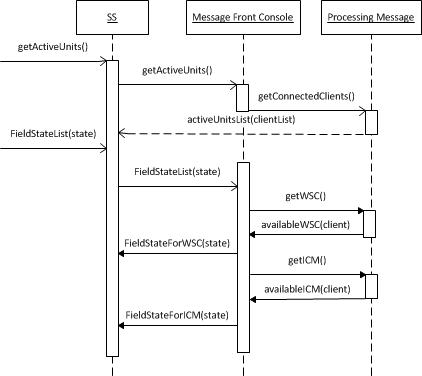
\includegraphics[width=8cm]{syySequenceDiagram.jpg}
  \caption{Representation of SYY squence diagram}\label{fig:syySequenceDiagram}
\end{figure}


\begin{figure}[h!]
  \centering
  % Requires \usepackage{graphicx}
  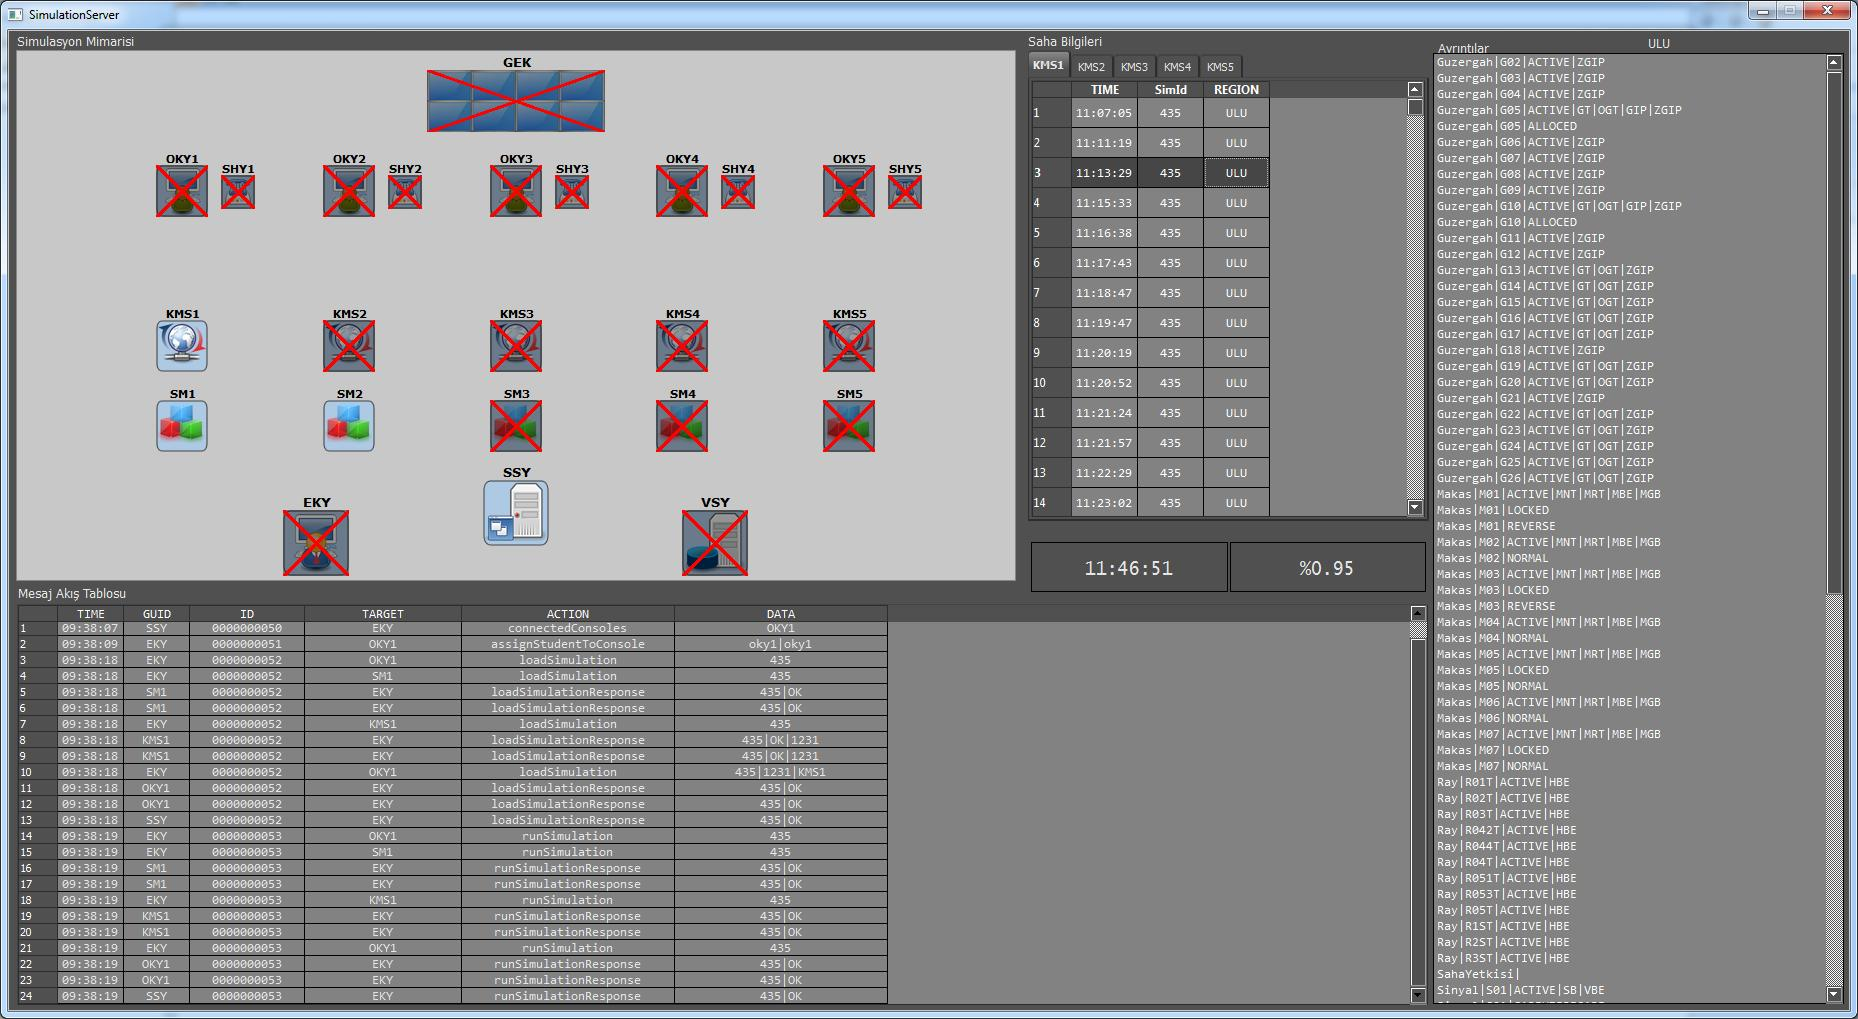
\includegraphics[width=8cm]{syygrafic.jpg}
  \caption{Representation of SYY UI}\label{fig:syygrafic}
\end{figure}




Hiyerarşik mesaj gönderimi bir mesajın, örneğin simülasyon yükleme mesajının öncelik sırasına göre her bir birime yollanması anlamına gelmektedir. Sıra ile yollanan her bir mesaj sonrasında olumlu cevap gelmesi durumunda bir sonraki ilgili birime mesaj iletilir. Bu zincir bir noktada kırılırsa sistem mesajı gönderen ilk birime olumsuz mesajı döndürür. Eğer mesaj zinciri tamamlanırsa olumlu mesajı iletilir.

\subsection{SM Simülasyon Motor Modülü}
\subsubsection{Sınıf Yapısı}
Simülasyon Motoru (SM) modülündeki Şekil \ref{fig:smgrafic}'de gösterilen ana sınıf SimMotor sınıfıdır. Bu sınıf Config, XmlUtility, SahaEventList, FTSimManager::FTSimMgr ve Communicator::Client sınıfları bünyesinde yaratıp kullanmaktadır. FTSimMgr Saha Trafik Simülasyon Yönetimi (FTS) modülünde tanımlıdır. SimMotor sınıfı FTSimMgr sınıfın sağladığı arayüz üzerinden anklaşman, saha ve trafik simülasyon modellerinde erişmektedir. Communicator modüllünde tanımlı Client sınıfı ise SimMotor sınıfına SimulationMessage mesajlaşma arayüz sağlamaktadır. SimMotorGui, SimMotor sınıfa debug ve test maksatlı grafik pencere arayüzü sağlamaktadır.

\begin{figure}[h!]
  \centering
  % Requires \usepackage{graphicx}
  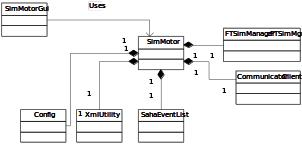
\includegraphics[width=8cm]{smgrafic.jpg}
  \caption{Representation of SM class diagram}\label{fig:smgrafic}
\end{figure}



\subsubsection{Mesajlaşma}
Simülasyon Sunucu Yönetimi (SSY) ilk başladığında 5 adet bağımsız Simülasyon Motoru (SM) proses yaratır. Bu SM proses’ler sayesinde 5 bağımsız simülasyon eşzamanlı olarak SSY tarafından kontrol edilmesine olanak sağlar. SSY SimulasyonMessage tür mesajarı SM ye aktarmaktadır. Bu tür mesajlar, simülasyon yükle, sümülasyon başlat tarzında üst seviye kontrol mesajlardır. SM bu mesajları Saha Trafik Yönetimi (FTS) simülasyon modüllerine iletmektedir. Simülasyon modülü bu mesajların gerektirdiği işlemleri tamamladığında SM’ye yanıt (olumlu veya olumsuz) vermektedir ve bu netice SSY ye geri bildirilmektedir.
LoadSimulation mesajı genel örnek olarak ele alınırsa; bu mesaj SM tarafından alındığında iki işlem tetiklemektedir. Birincisi, senaryo da oynatılması gereken önceden programlanmış olaylar veritabanından okunuyor ve Saha Event List (SEL) listesine yüklenmektedir. Bu olayların her biri bir Saha Event (SE) olarak tanımlanmıştır. 
İkinci işlem ise FTS ve onun bünyesindeki Saha Simülasyon (SS) modeli, Anklaşman Simülasyon (AS) modeli ve Trafik Simülasyon (TS) modelini ilgili senaryonun teknik parametrelerini veritabanından yüklemesi ve simülasyon başlatma durumu için hazırlanması.
Simülasyon Running durumundayken SEL deki sıralanmış SE olaylar simülasyon zamanına göre FTS modülüne işlenmek için aktarılmaktadır. Bu mekanizma bir senaryonun müdahalesiz olarak işlenmesini sağlamaktadır. Ancak bir simülasyon ayrıca eğitmen tarafından müdahale edilmesine izin vermektedir. Eğitimen, Eğitmen Saha Müdahale (ESM) aracı kullanarak manuel Saha Event yaratabilir. Bu manuel olarak yaratılan SE olaylar SM’ye anlık olarak iletdiğinde SE olayı SEL listesinin başına eklemektedir ve böylelikle simülasyon’un sonraki çevriminde hemen işlenmesi sağlanmaktadır. Bütün bu akış Şekil \ref{fig:smCommunicationDiagram}'deki diagramda gösterilmiştir.

\begin{figure}[h!]
  \centering
  % Requires \usepackage{graphicx}
  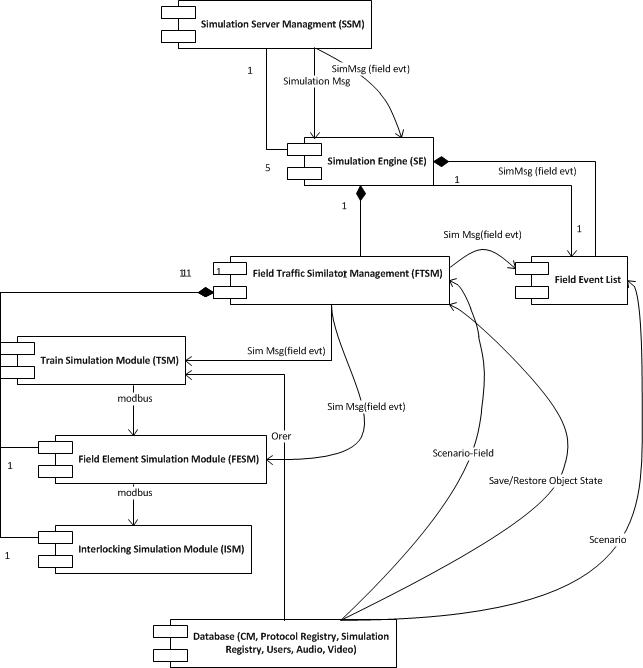
\includegraphics[width=8cm]{smCommunicationDiagram.jpg}
  \caption{Representation of SM Comminication diagram}\label{fig:smCommunicationDiagram}
\end{figure}

\subsubsection{SD Simülasyon Destek ve Mesajlaşma Modülü}

Şekil \ref{fig:RepresentationSDDiagram}'de görüldüğü gibi Simülasyon Destek ve Mesajlaşma modülü proje içerisinde birbirinden fiziksel olarak bağımsız fakat haberleşme ve etkileşim içinde olan birimlerin birbirleri ile olan haberleşmesini sağlamaktadır.
Temel sunucu istemci mimarisi üzerine kurulmuş haberleşme modülü projeye özgü bağlantı kopukluğu kontrolü, tekil bağlantı özelliği, XML tabanlı mesaj kontrolü gibi özellikler eklenerek projeye özgü protokol kuralları çerçevesinde tasarlanmıştır.
Mesajlaşma ve iletişimi sağlayacak olan ana modül iki modda çalışabilmektedir. Bu modalardan ilki Server yani sunucu mod iken diğer mod ise Client yani istemci modüldür. Sunucu modda çalıştırıldığında belirli bir bağlatı portu üzerinden haberleşmenin sağlandığı bu sistem modda diğer yani İstemci modda diğer sistemlerin bağlanılması beklenmektedir. 

\begin{figure}[h!]
  \centering
  % Requires \usepackage{graphicx}
  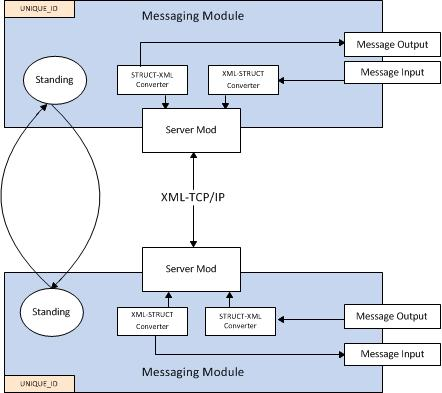
\includegraphics[width=8cm]{RepresentationSDDiagram.jpg}
  \caption{Representation of SD  diagram}\label{fig:RepresentationSDDiagram}
\end{figure}

İstemci mod bağlantı esnasında hedef sunucu bilgilerini ve kendisini tanıtan tekil eşsiz bir ID ile erişimi sağlayacaktır. Bu bağlantıları eşsiz hale getirmek için IP numaraları kullanılmayacaktır. Çünkü aynı makina üzerindeki farklı uygulamalar birbirleri ile sunucu üzerinden haberleşme yeteneğine sahip olmalıdır. Aynı ID ile birden fazla erişim denemesi yapıldığında sistem 2. sistemin bağlantı denemesini “Kullanımdaki bir ID” uyarsıyla reddedecektir. 
Şekil \ref{fig:SDDiagram}'de görüldüğü gibi yine bir sunucuya bağlı olan tüm istemciler o sunucuya periyodik olarak sunucuya bağlı oldukları yani ayakta oldukları bilgisini yollarlar. Ters açıdan bakıldığında sunucu da kendisine bağlı olan tüm istemcilere çalışır yani ayakta olduğu bilgisini periyodik olarak bildirmektedir. Bu sayede sistemdeki tüm elemanların bağlantı kontrolü gerçekleştirebilecektir. 


\begin{figure}[h!]
  \centering
  % Requires \usepackage{graphicx}
  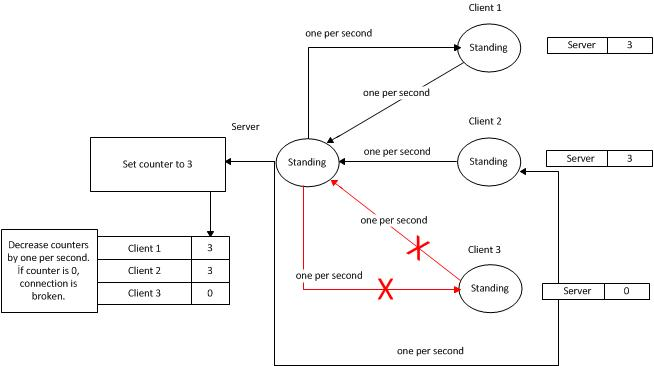
\includegraphics[width=8cm]{SDDiagram.jpg}
  \caption{Representation of SD  diagram}\label{fig:SDDiagram}
\end{figure}




\section{Training Environment}

\subsection{ÖK Öğrenci Konsolu}

Öğrenci Konsolu (ÖK) bir Öğrenci Bilgisayarı (ÖBÜ) ve bir Sesli Haberleşme Cihazından (SHC) alt donanım bileşenlerden oluşmaktadır. ÖK’nin yapısı Şekil \ref{fig:ogrenci}'de gösterilmiştir.
Öğrenci Bilgisayarı bilgisayar kasa, fare, klavye ve LCD ekran donanımlardan oluşmaktadır. Bilgisayar üzerinde Windows 7 işletim sistemi kuruludur. Öğrenci Konsol Yönetimi (ÖKY) yazılım modülü üst seviye modül olup konsolunun genel işlevlerinden sorumludur. Dispeçer arayüz uygulamasını KM Client (KMC) modülü gerçekleştiriyor. Ekranların video görüntü kayıtları Video Kayıt Altyapı (VKA) modülü tarafından gerçekleştiriliyor.
Sesli Haberleşme Cihazı dispeçerin sesli iletişimini sağlamak için gerekli mikrofon, kulaklık veya telefon ahize ile donatılacaktır. Üzerinde çalışan Sesli Haberleşme Yazılım Modülü (SHY) eğitim amaçlarına uygun biçimde arama yapmayı, aranmayı destekleyecektir. 

\begin{figure}[h!]
  \centering
  % Requires \usepackage{graphicx}
  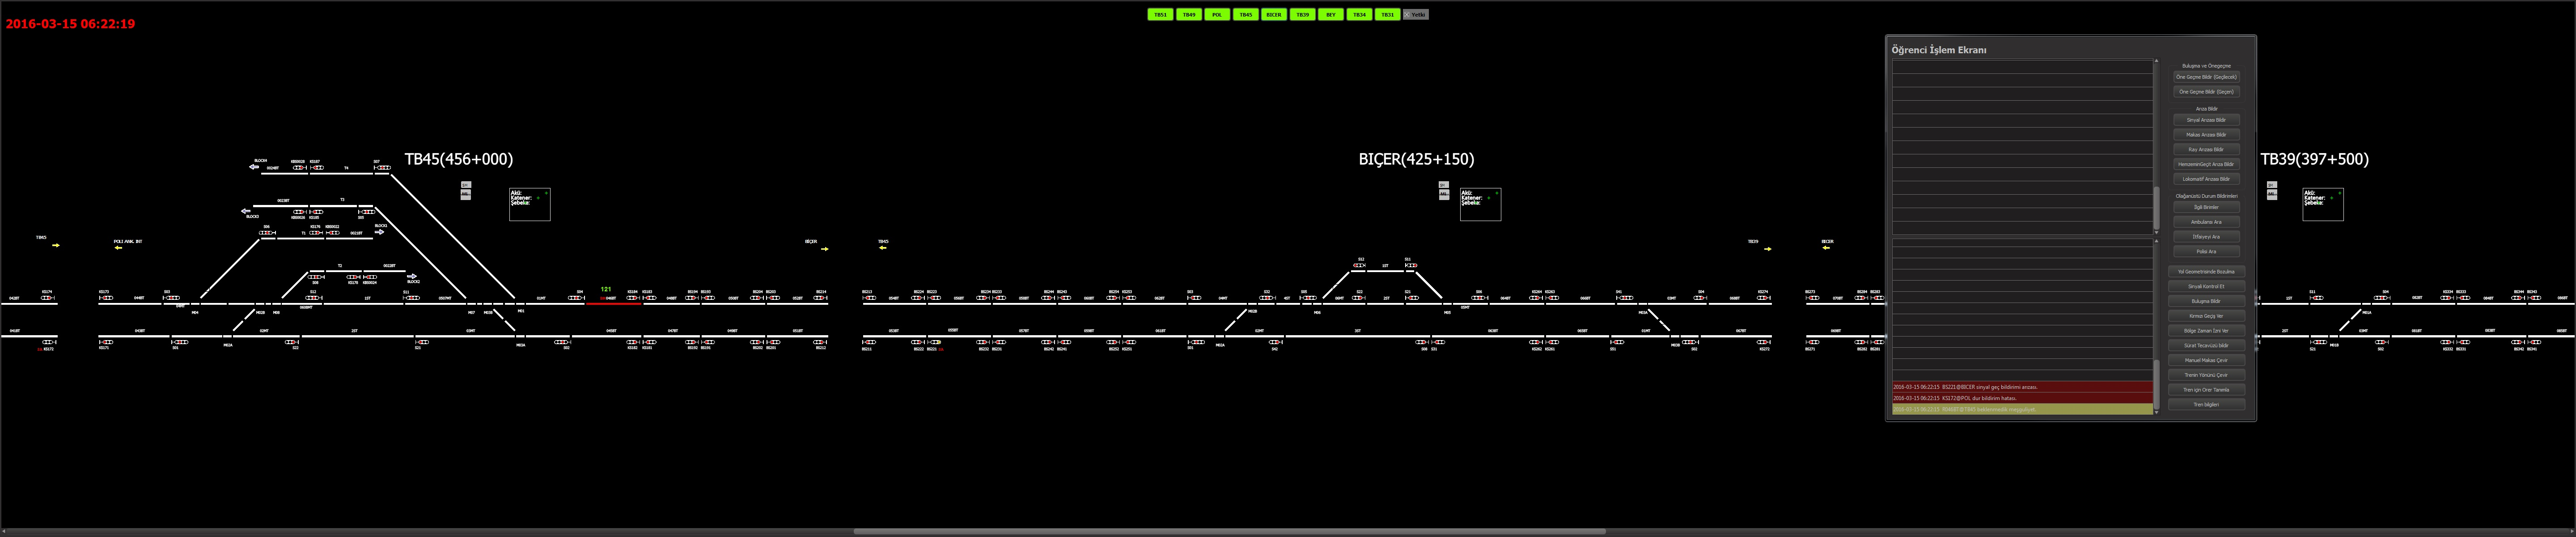
\includegraphics[width=8cm,height=5cm]{ogrenci.jpg}
  \caption{Representation of Dispatcher Console}\label{fig:smclass}
\end{figure}



\subsection{GEK Geniş Ekran Konsolu}

Geniş Ekran Konsolu (GEK) bir Geniş Ekran Bilgisayar Ünitesi (ÖBÜ) ve bir Geniş Ekran Duvar Ünitesi (GDÜ) donanım bileşenlerden oluşmaktadır.GEK’in yapısı Şekil 3 de gösterilmiştir.
Geniş Ekran Bilgisayar Ünitesi (GBÜ) çok çıkışlı ekran kartı ile donatılmış olup, her çıkış Geniş Ekran Duvar ünitesinin birer ekranına bağlıdır. Bilgisayar üzerinde Geniş Ekran Konsol Yönetimi (GKY) yazılımı çalışmaktadır. Bu yazılım Dispeçer arayüz uygulaması olan KM Client (KMC), Video Kayıt Altyapı (VKA) ve Video Geri Oynatma Aracı (VGO) modüllerin çalıştırılması ve kontrol edilmesinden sorumludur.
Sesli Haberleşme Cihazı eğitmenin sesli iletişimini sağlamak için gerekli mikrofon, kulaklık veya telefon ahize ile donatılacaktır. Üzerinde çalışan Sesli Haberleşme Yazılım Modülü (SHY) eğitim amaçlarına uygun biçimde arama yapmayı, aranmayı destekleyecektir.
Şekil \ref{fig:genisekranSonuc}'de geniş ekrana ait deney sonucundaki ekran göüntüsü görülmektedir.


\subsection{Eğitmen Konsolu}

Eğitmen Konsolu (EK) bir Eğitmen Bilgisayar Ünitesi (EBÜ) ve bir Geniş Ekran Duvar Ünitesi (GDÜ) donanım bileşenlerden oluşmaktadır. EK’nin yapısı Şekil 4 de gösterilmiştir.
Eğitmen Bilgisayar Ünitesi (EBÜ) kasa, fare, klavye ve LCD ekran donanımlardan oluşmaktadır. Bilgisayar üzerinde Windows 7 işletim sistemi kuruludur. Bilgisayar üzerinde Eğitmen Konsol Yönetimi (EKY) yazılımı çalışmaktadır. Bu yazılım  Eğitmen Simülasyon Yönetim (ESY), Eğitmen Saha Müdahale (ESM), ve Video Geri Oynatma (VGO) modüllerin çalıştırılması ve kontrol edilmesinden sorumludur.
Geniş Ekran Duvar Ünitesi (GDÜ) iki satır dört sütün düzenine göre yerleştirilmiş 8 LCD ekranlık görüntüleme duvardır. Şekil \ref{fig:egitmenSonuc}'de eğitmen paneli ile yapılan deneye ait ekran görüntüsü yer almaktadır.


\subsection{SSÜ Simülasyon Sunucu Ünitesi}

RAYTES projesinde tüm mesajlaşma koordinasyonu sağlamak amacıyla Simülasyon Sunucu Ünitesi uygulaması kullanılacaktır. Endüstriyel bir sunucu bilgisayarda koşacak uygulama proje ekibi tarafından geliştirilecektir. Uygulamanın temel işlevleri simülasyon bileşenleri arasında mesajlaşma senkronizasyonunu ve koordinasyonu sağlamak, sistemin çalışmasını tüm mesaj akışlarını görüntülemek, simülasyon altyapısını oluşturan diğer sunucu taraflı bileşenlerin ayağa kaldırılmasını sağlamak, simülasyon bileşenlerin bağlantı bilgilerini tutmak ve bunları diğer bileşenlerle paylaşmak gibi görevlerdir. Simülasyon sisteminin tüm aktif bileşenleri Simülasyon sunucusuna doğrudan ya da dolaylı olarak bağlı bulunacaktır.
\subsection{Editör Analiz Konsolu}

Editör Analiz Konsolu (EAK) bilgisayar kasa, fare, klavye ve LCD ekran donanımlardan oluşmaktadır. EAK’nin yapısı Şekil 7 da gösterilmiştir.
Bilgisayar üzerinde Windows 7 işletim sistemi kurulu olup Senaryo Editör Aracı (SED), Performans Analiz Aracı (PA), Kullanıcı Yönetim Aracı (KYA), Öğrenci Eğitim Kayıtları Aracı (ÖEK) ve Video Geri Oynatma Aracı (VGO) yazılım modüller çalışmaktadır.
EAK simülasyon öncesi senaryoların hazırlanması, kullanıcıların tanımlanması, ve simülasyon sonrası eğitim performans analizi ve öğrenci eğitim kayıtlarını incelemek için kullanılmaktadır. Dolaysıyla bu konsol simülasyon eğitimi esnasında değil “off-line” kullanılmaya yöneliktir.

\subsection{Train Graph}


Raytes Projesi kapsamında geliştirilen Trengraf bileşeni, tren hareket kayıtlarının (TrainEvent) sorgulanarak grafik üzerinde çeşitli seçenekler ile gösterimini sağlayan bir veri analiz aracıdır.
74 de örnek bir ekran görüntüsü verilmiştir. Sorgu sonucunda trenlerin bloklardan geçiş hareketleri rahatlıkla izlenebilmektedir. 


\begin{itemize}
\item Eğrinin solundaki çizgi ile işaretlenmiş noktalar trenin bloklara girişini,
\item Eğrinin sağındaki çizgi ile işaretlenmiş noktalar trenin bloklardan çıkışını,
\item İki çizgi arasında kalan transparan boyalı alan ise giriş-çıkış arasındaki zaman farkını, yani trenin o blokta ne kadar kaldığını ifade etmektedir.
\end{itemize}

Bu seçeneklerin hangilerinin gösterileceği kullanıcı tarafından seçilebilmektedir.
Şekil \ref{fig:trenGrapSonuc}'de tren grafa ait çalıştırılan deney sonucundaki ekran göüntüsü görülmektedir.


\section{EXPERIMENT RESULT}
Geliştirdiğimiz dağıtık yapılı 5 öğrencinin aynı anda eğitim alabildiği RAYTES projemizi 2 şekilde test ettik. Bunlardan ilki 20 tren ve tek simülasyon 5 kullanıcı yetkisi dahilinde 1 saatlik seneryoda eğitim aldılar. Toplam RAM ve CPU kullanımı Şekil \ref{fig:hepsibir}'de gösterilmiştir


\begin{figure}[h!]
  \centering
  % Requires \usepackage{graphicx}
  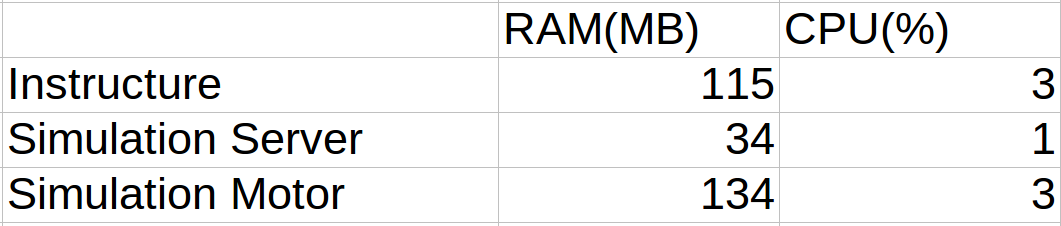
\includegraphics[width=8cm]{hepsibir.png}
  \caption{Tek simülasyon ve 5 farklı öğrenci ile yapılan eğitime ait modüllerin kaynak kullanımını göstermektedir}\label{fig:hepsibir}
  
\end{figure}

Diğer testimizde 1'er saatilik 5 ayrı simülasyon ve her simülasyona bir öğrenci atandı. Bu şekilde eğitim aldılar. Toplam RAM ve CPU kullanımı Şekil \ref{fig:hepsiayri}'de gösterilmiştir

\begin{figure}[h!]
  \centering
  % Requires \usepackage{graphicx}
  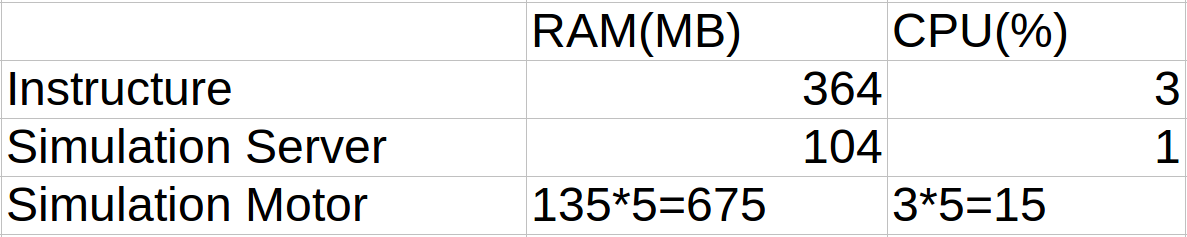
\includegraphics[width=8cm]{hepsiayri.png}
  \caption{5 farklı simülasyon ve 5 farklı öğrenci ile yapılan eğitime ait modüllerin kaynak kullanımını göstermektedir}\label{fig:hepsiayri}
  
\end{figure}

Deneyler sonucunda elde edilen tren hareketlerini gösteren tren graf şekildeki gibi olmaktadır. 
\begin{figure}[h!]
  \centering
  % Requires \usepackage{graphicx}
  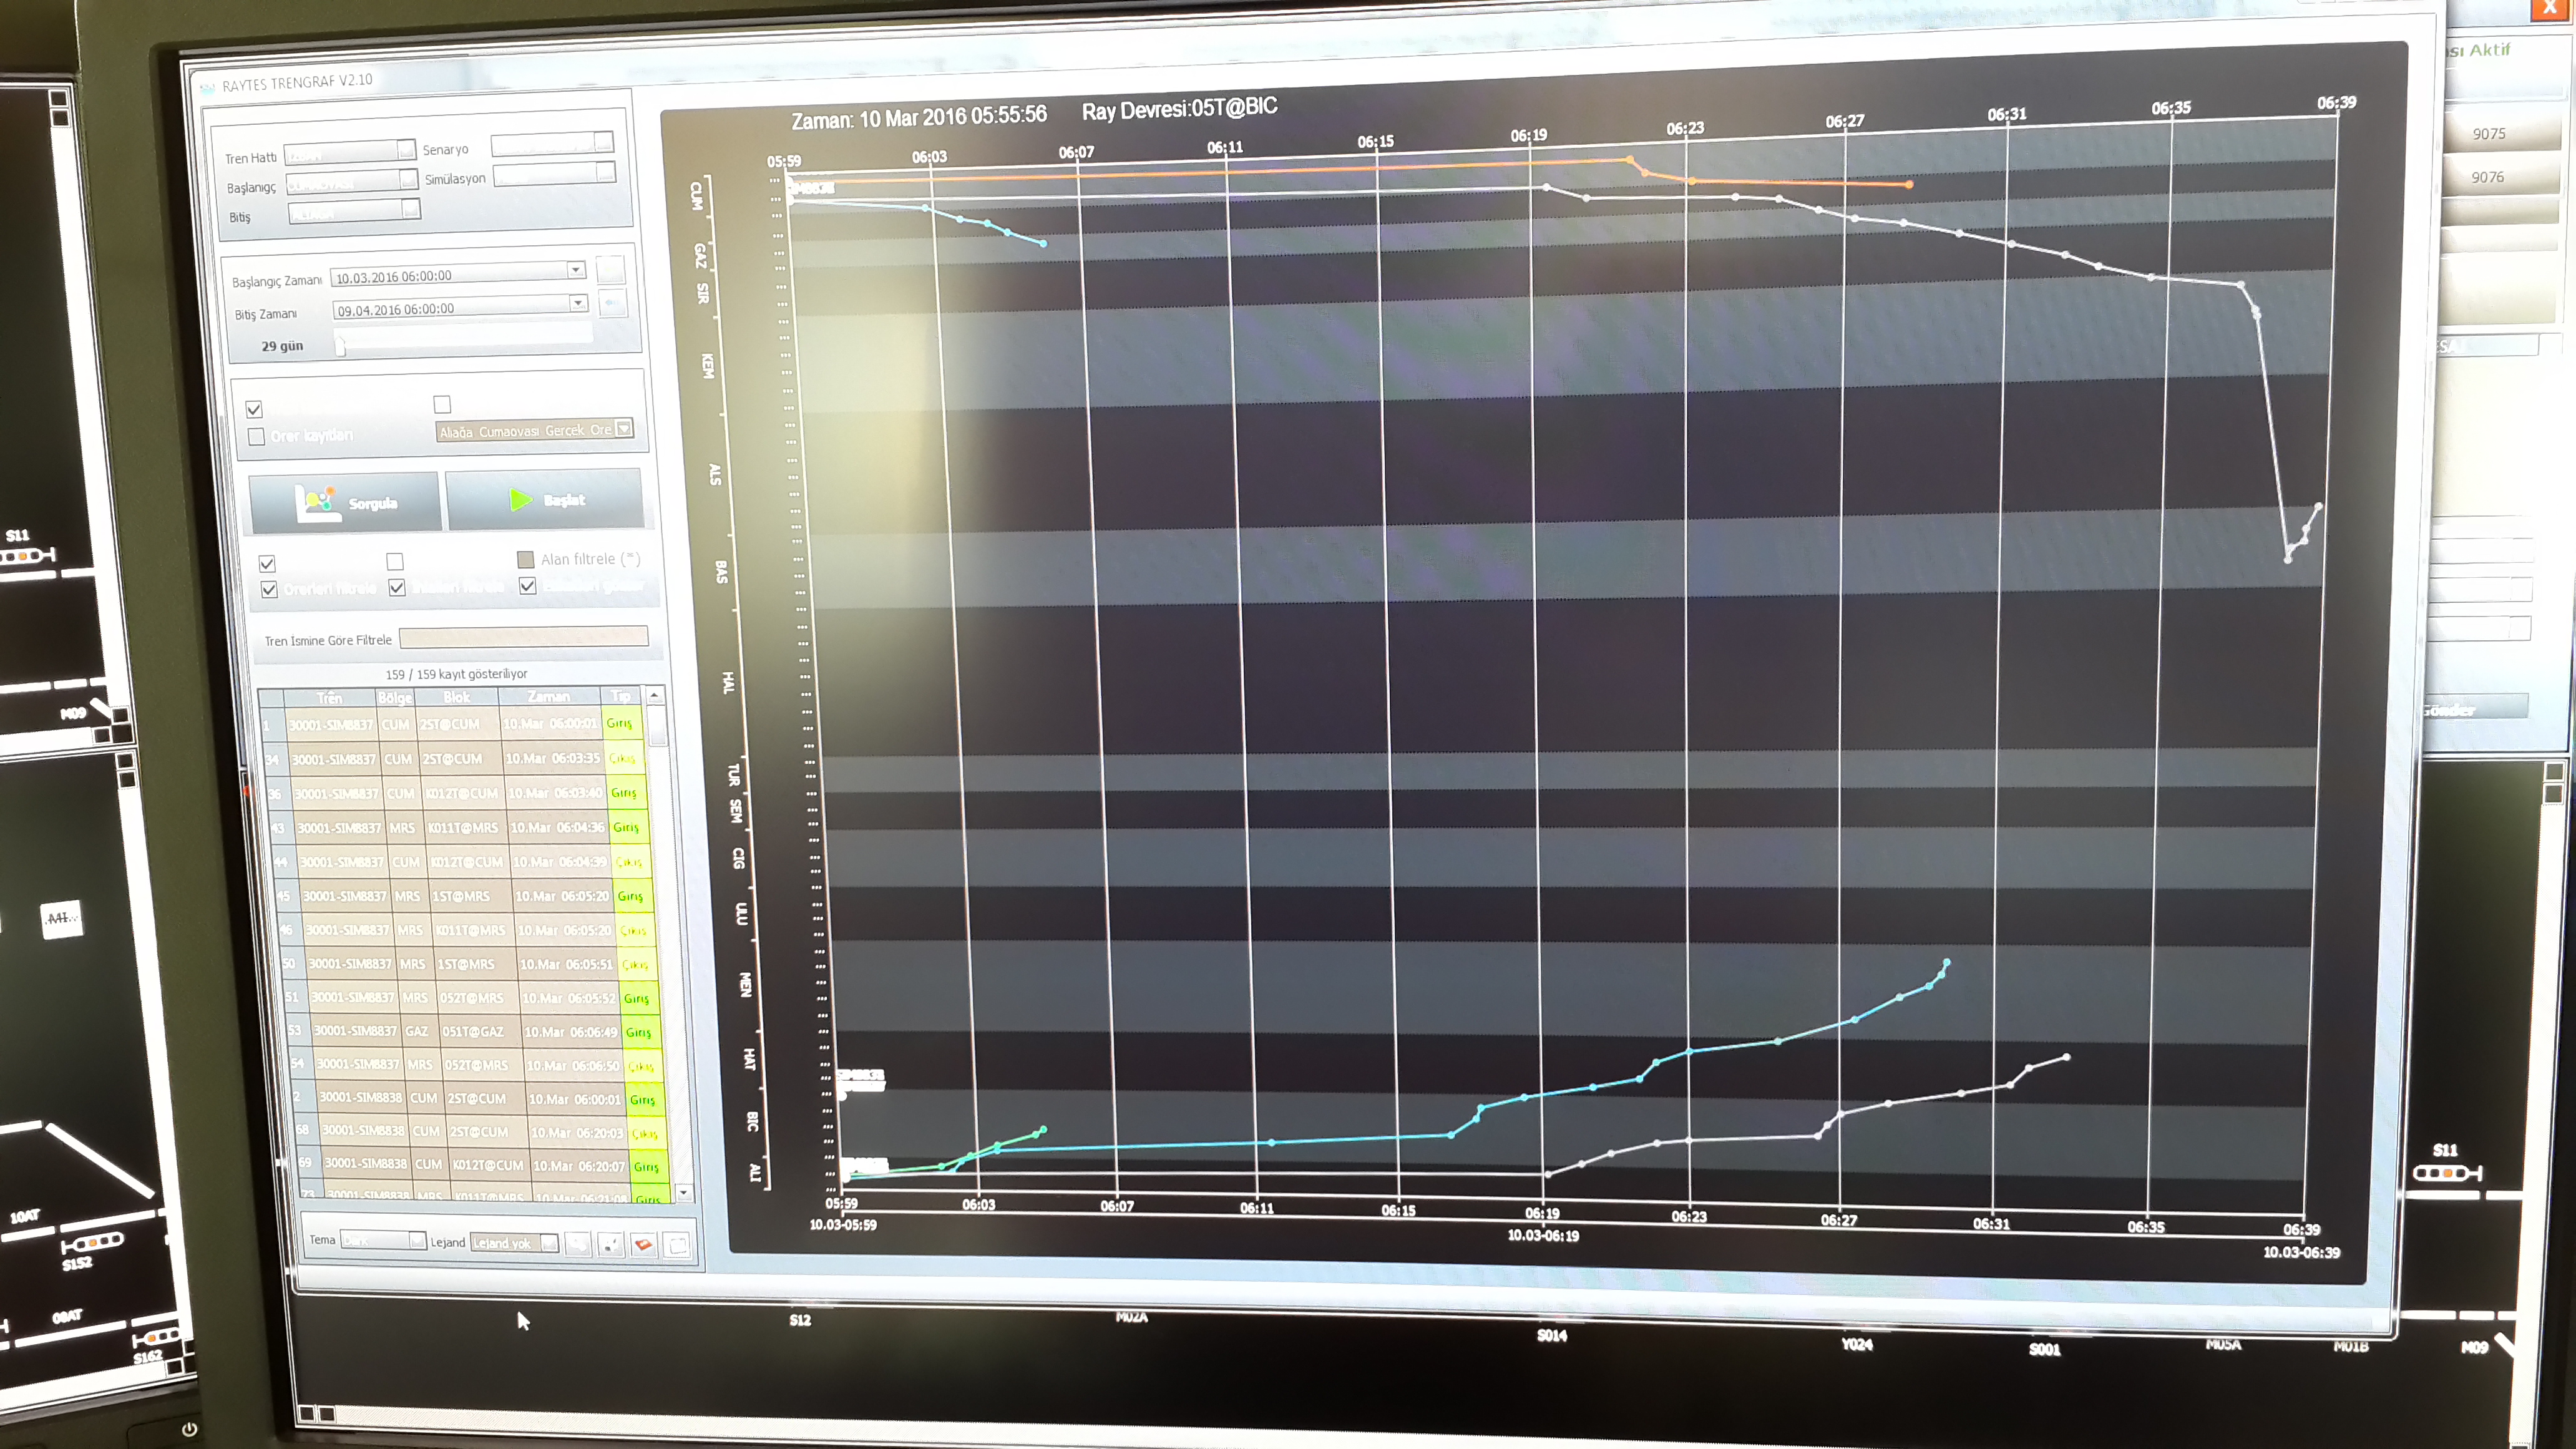
\includegraphics[width=8cm]{trenGrapSonuc.jpg}
  \caption{Tren hareketlerinin gösterimi}\label{fig:trenGrapSonuc}
  
\end{figure}
\begin{figure}[h!]
  \centering
  % Requires \usepackage{graphicx}
  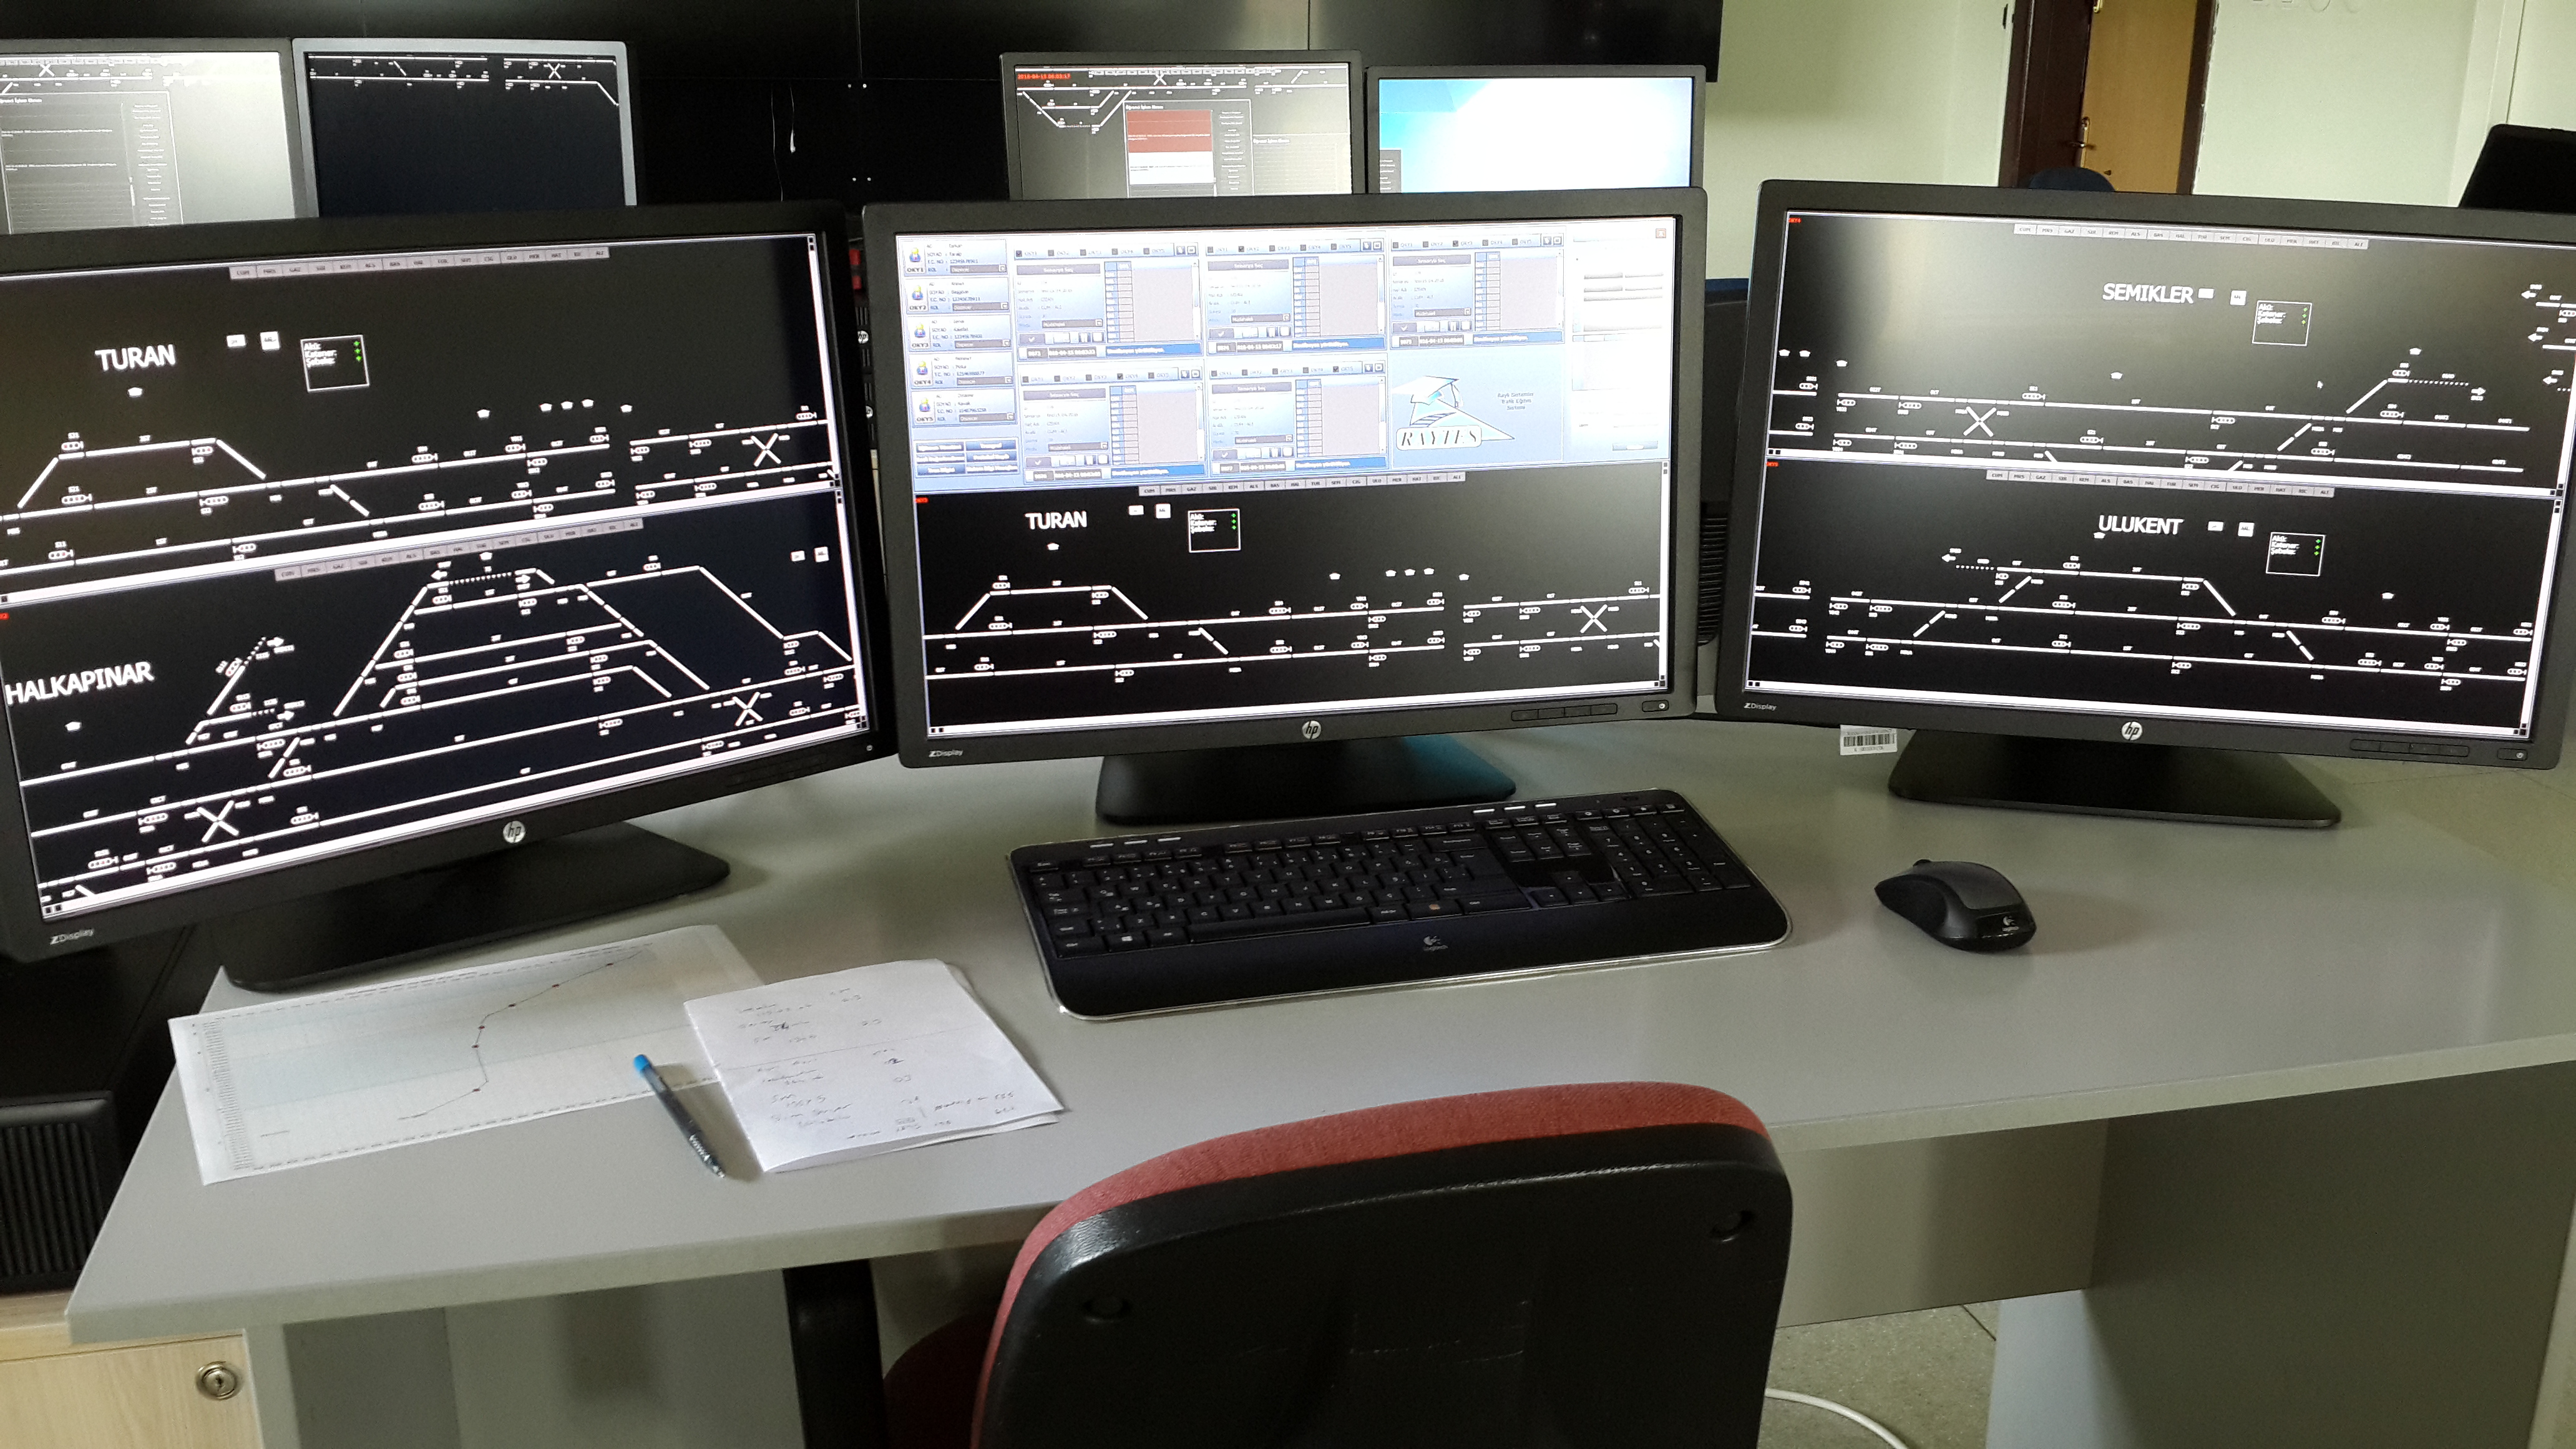
\includegraphics[width=8cm]{egitmenSonuc.jpg}
  \caption{5 farklı simülasyon ve 5 farklı öğrenci ile yapılan eğitimin eğitmen konsolunda gösterimi}\label{fig:egitmenSonuc}
  
\end{figure}
\begin{figure}[h!]
  \centering
  % Requires \usepackage{graphicx}
  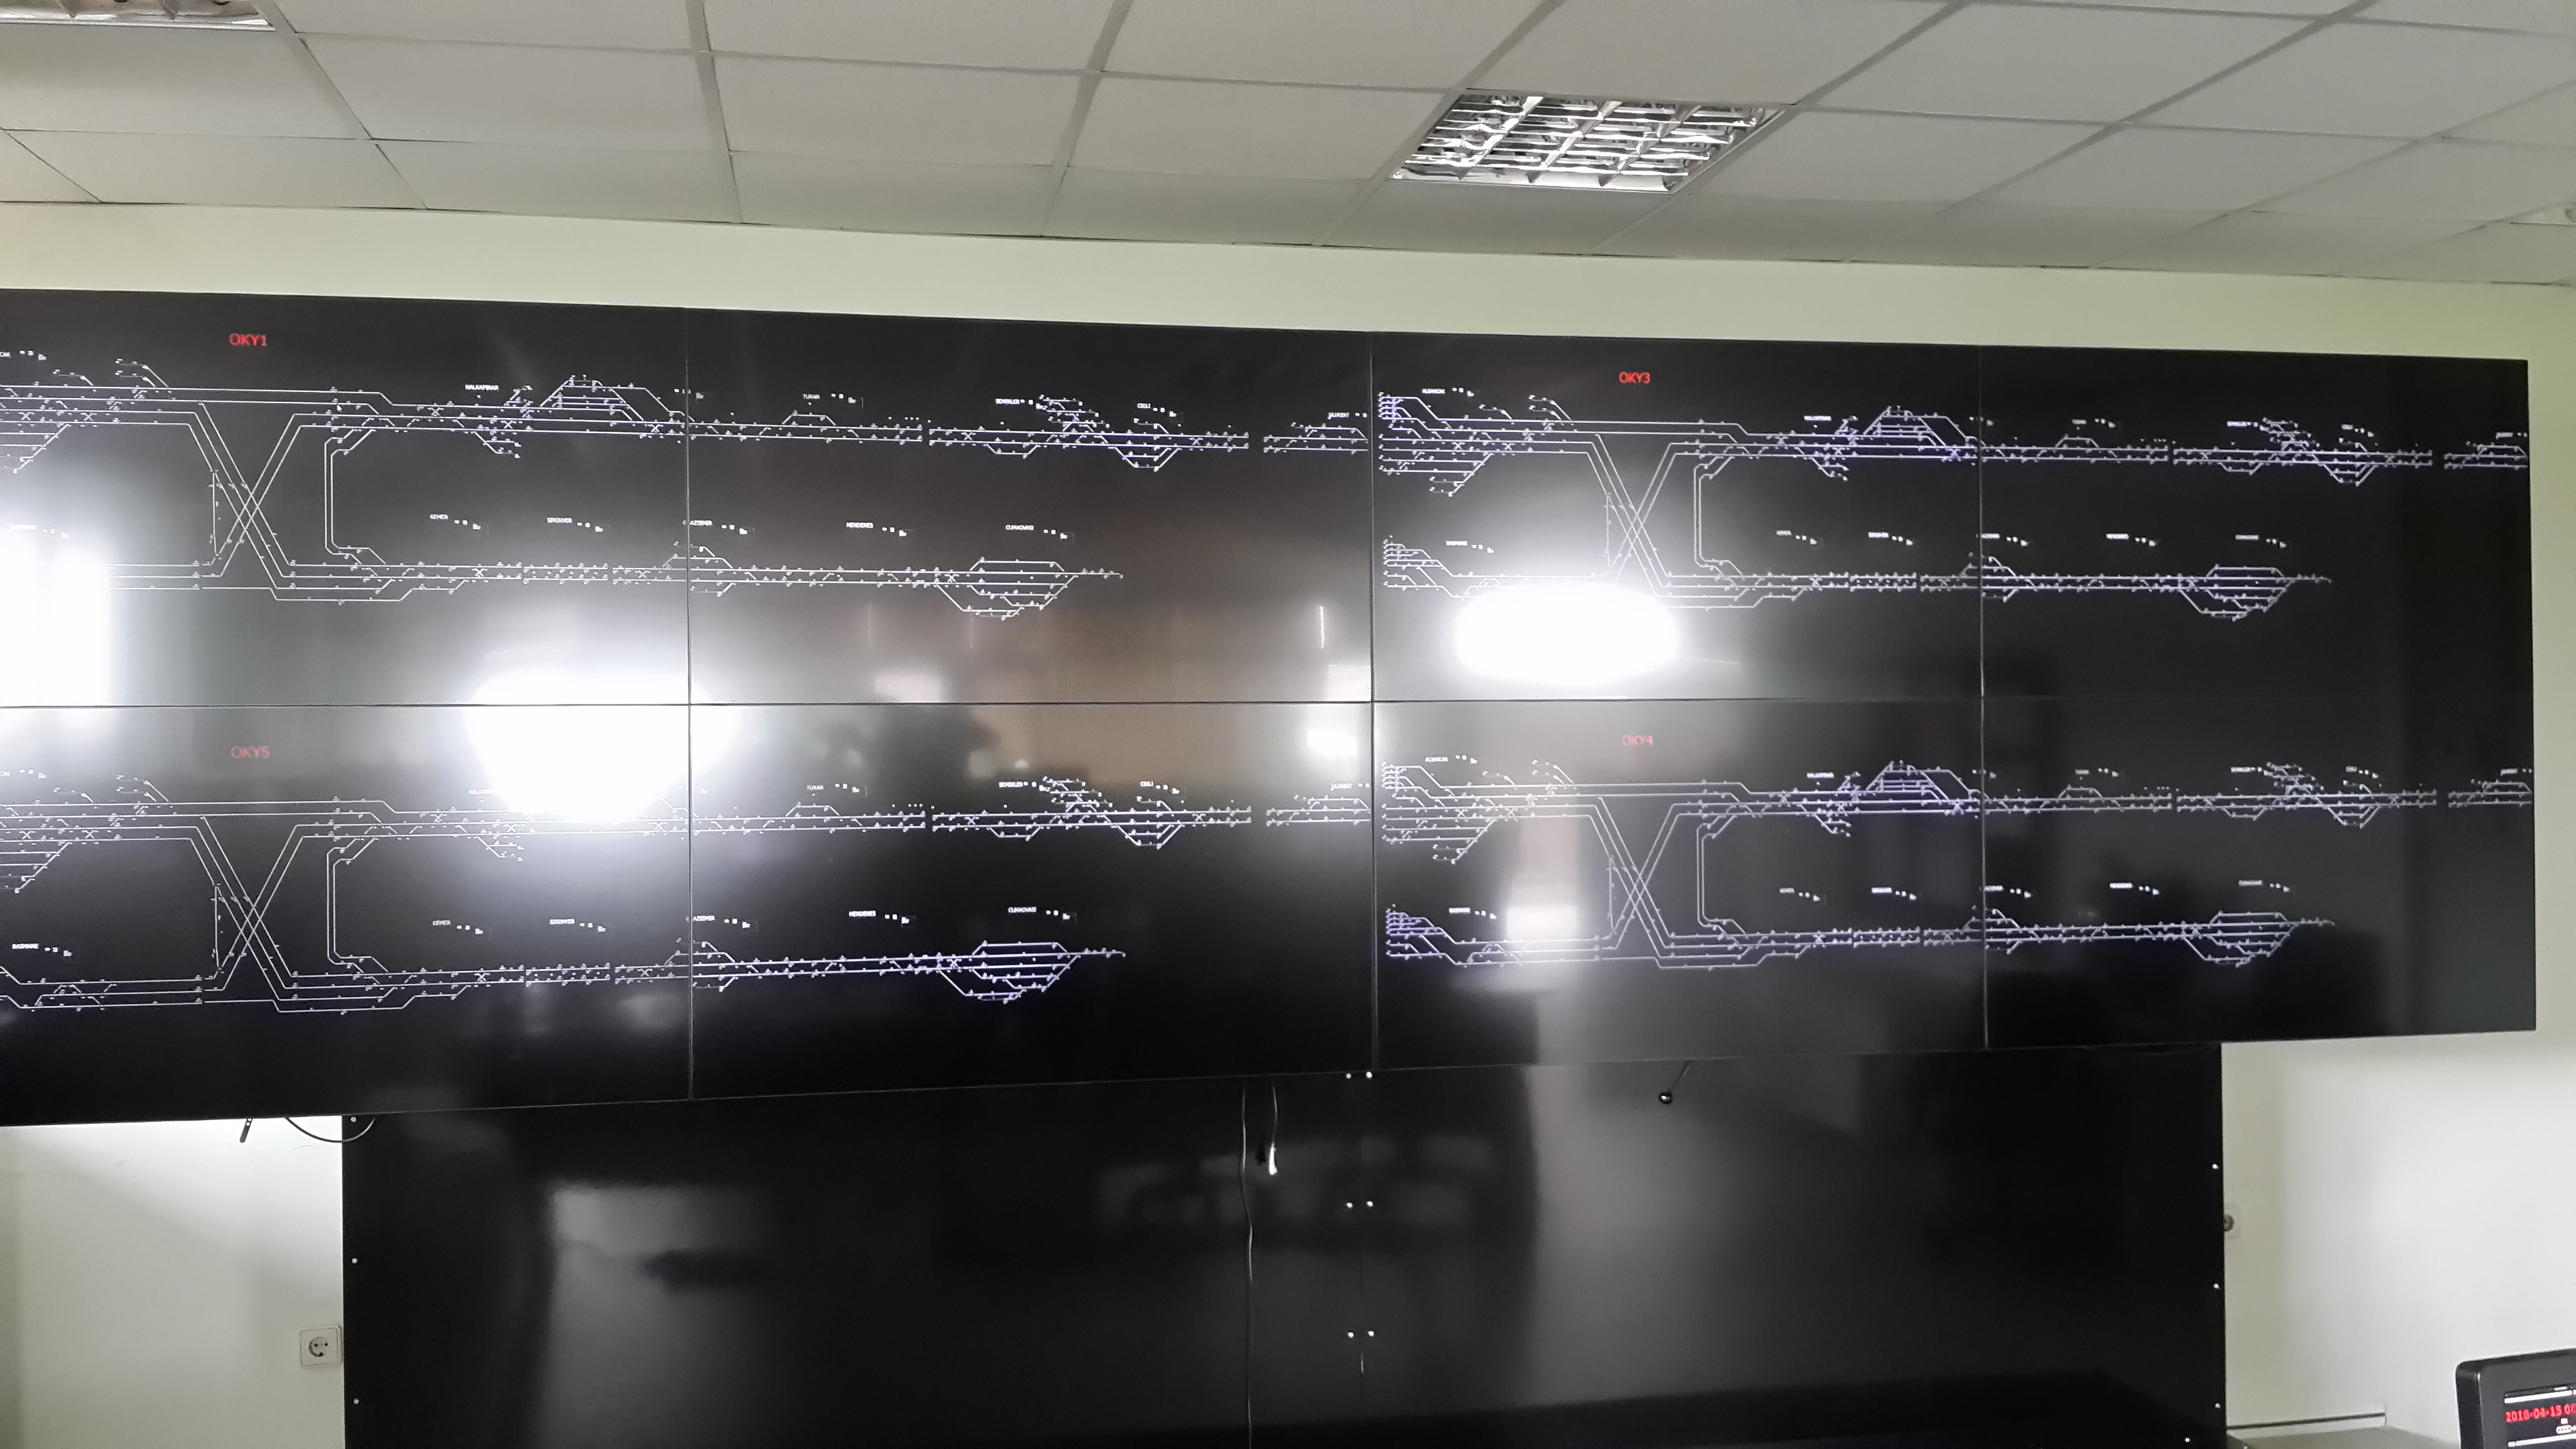
\includegraphics[width=8cm]{genisekranSonuc.jpg}
  \caption{4 farklı kullanıcıya ait ekran görüntülerinin geniş ekranda gösterimi}\label{fig:genisekranSonuc}
  
\end{figure}


\section{Conclusion}
Computer Simulations can be considered as a powerful tools for learning such as analysing, designing, and interacting. Especially in the vital criticality level it has become more important tools such as train traffic simulation.
The most important purpose of the train control system to prevent train collisions with other trains, keeping them in safe range.

The purpose of this study is to provide train traffic control in a distributed simulation system. The system consists of an instructor support five students and a scenario-editor. The system use real train route model located in Turkey.  During the simulation, dispatchers console can controls train traffic which have different  size and speed in system. Success in educational outcomes can be measured. Instructor console make decisions about the organization of teaching and learning experiences, classroom management, and responses to individual students. The user is able to monitor and track the progress of five targeted students throughout the course of the simulation.





% conference papers do not normally have an appendix


% use section* for acknowledgment
\section*{Acknowledgment}


This work has been conducted within Rail Transit systems Simulation Research Lab- project (project number 3920-S513000) for Turkish State Railways, which is part of the Rail Transit Systems research program funded by The National Research Institute of Electronics and Cryptology (TUBITAK BILGEM). We thank all project partners for their work and contributions to the project.






% trigger a \newpage just before the given reference
% number - used to balance the columns on the last page
% adjust value as needed - may need to be readjusted if
% the document is modified later
%\IEEEtriggeratref{8}
% The "triggered" command can be changed if desired:
%\IEEEtriggercmd{\enlargethispage{-5in}}

% references section

% can use a bibliography generated by BibTeX as a .bbl file
% BibTeX documentation can be easily obtained at:
% http://mirror.ctan.org/biblio/bibtex/contrib/doc/
% The IEEEtran BibTeX style support page is at:
% http://www.michaelshell.org/tex/ieeetran/bibtex/
%\bibliographystyle{IEEEtran}
% argument is your BibTeX string definitions and bibliography database(s)
%\bibliography{IEEEabrv,../bib/paper}
%
% <OR> manually copy in the resultant .bbl file
% set second argument of \begin to the number of references
% (used to reserve space for the reference number labels box)
\begin{thebibliography}{1}

\bibitem{FRISO}
A. D. Middelkoop and L. Loeve, “Simulation of traffic management with FRISO,” 2006, vol. 1, pp. 501–509.

\bibitem{ICVES}
M. Baohua, J. Wenzheng, C. Shaokuan, and L. Jianfeng, “A computer-aided multi-train simulator for rail traffic,” in IEEE International Conference on Vehicular Electronics and Safety, 2007. ICVES, 2007, pp. 1–5.
 
 
 

\end{thebibliography}




% that's all folks
\end{document}


